% BMC Psychology major revision, v0.4, 2 October 2026.
% Springer Nature article template, version 3.1 (December 2024).
% Author-identifying and funding fields remain explicit placeholders.
\documentclass[pdflatex,sn-vancouver-num]{sn-jnl}

\usepackage{graphicx}
\usepackage{booktabs}
\usepackage{tabularx}
\usepackage{array}
\usepackage{amsmath,amssymb}
\usepackage{url}
\usepackage{placeins}
\usepackage[switch]{lineno}
\usepackage{setspace}

\raggedbottom
\unnumbered

\begin{document}
\doublespacing
\linenumbers

\title[When early personal baselines lose relevance]{When early personal baselines lose predictive relevance: cross-timescale evidence from repeated psychological self-reports}

\author[1]{\fnm{Runqing} \sur{Liao}}\email{202411055222@stu.hstc.edu.cn}
\author*[1]{\fnm{Zhining} \sur{Wang}}\email{mathwangzhining@163.com}
\affil*[1]{\orgdiv{School of Mathematics and Statistics}, \orgname{Hanshan Normal University}, \orgaddress{\city{Chaozhou}, \postcode{521041}, \country{China}}}

\abstract{\textbf{Background:} Repeated psychological assessments are often interpreted relative to a person's earlier reports. This reference may become unrepresentative as states, contexts, or response processes change. We tested whether an early baseline became less useful than an equally sized recent history and whether any advantage was specific to one updating rule.

\textbf{Methods:} Secondary analyses used three longitudinal datasets: Dejonckheere/openESM ($n=100$), the College Experience Study (CES; $n=105$), and Marian/openESM ($n=145$). For each later report, we compared the mean of the first eight complete reports (B8) with the eight most recent complete reports (L8). Outcomes comprised five momentary affect or stress ratings, Patient Health Questionnaire-2 scores, and two momentary depression-related items. Participant-bootstrap intervals and temporal null models assessed uncertainty and ordering. Sensitivity analyses varied window length, modelled observation probability, separated CES recall periods, and reset the calibration origin. A semi-synthetic stress test examined sustained worsening.

\textbf{Results:} L8 reduced participant-balanced mean absolute error relative to B8 for all eight analysed outcomes (9.97\%--29.80\%). For the four primary outcomes, circular-shift tests passed the Bonferroni threshold ($p_{\mathrm{MC}}=0.002$--$0.006$). The error advantage remained directionally stable across window and observation-process checks. After resetting the calibration origin, late-origin advantages remained for stress, PHQ-2, and depressed mood but were inconclusive for sadness; age slopes attenuated and were not consistently positive. A fixed exponentially weighted mean was 2.05\%--3.31\% more accurate than L8. In the structural stress test, L8 retained 16.4\% of an imposed sustained deviation and a 50:50 anchored rule retained 58.2\%.

\textbf{Conclusions:} In these three selected samples, early start-anchored baselines were less predictive than recent history, but part of the apparent age gradient was specific to the original study start. Personal references should be audited for when and how they were established without assuming a universal decay law. Updating improved short-horizon prediction while attenuating imposed sustained deviations; clinical use requires prospective outcomes and externally defined action thresholds.}

\keywords{ecological momentary assessment; intensive longitudinal data; personal baseline; psychological measurement; depression; affect; within-person change; nonstationarity; prediction}

\maketitle

\section{Background}

When psychological states are measured repeatedly, a person's earlier answers provide a natural point of reference. A sadness score of 40, for example, may carry a different meaning for someone who usually reports very little sadness than for someone whose reports are commonly higher. Personal baselines are therefore attractive in longitudinal research: they can reduce stable differences between people and make current observations interpretable relative to the person's own history. This logic underlies many idiographic, ecological momentary assessment (EMA), and personalised prediction approaches \cite{ref1,ref2,ref3}.

The usefulness of a personal reference nevertheless depends on an assumption that is often left implicit: earlier observations must remain representative of the person at the time of prediction. Psychological states vary within individuals, and their dynamics depend on the time scale of measurement \cite{ref4,ref5,ref6}. A baseline established near the beginning of a study may reflect a transient period, an earlier academic or social context, or a different phase of symptoms. As time passes, the baseline can become statistically precise about the past while becoming less relevant to the present. We refer to this problem as loss of baseline freshness. The term is descriptive: it does not presume that time itself causes psychological change or that a particular latent process is responsible.

Existing longitudinal models provide several ways to use personal history. A fixed person mean emphasizes stable differences, the most recent observation emphasizes short-term continuity, and time-series or multilevel models combine longer and shorter histories \cite{ref2,ref5,ref7}. Studies using smartphones and wearables have likewise reported heterogeneous benefits from person-specific modelling \cite{ref8,ref9,ref10}. Temporal windows can change which psychological associations are visible \cite{ref18}, and leakage-prone validation can make complex mobile-health models look better than simple heuristics \cite{ref19}. Recent work has therefore framed individual baselines as forecasting rules whose validity depends on the task, person, context, and updating scheme \cite{ref20}. That framework motivates auditing a baseline, but it does not answer the narrower measurement question tested here: whether two arithmetic means built from the same number of reports differ because one is anchored to the study start and the other is temporally local. A recent-history predictor usually has access to more observations or a more flexible model. Better prediction can then be attributed to information quantity or model complexity rather than to the temporal location of the personal reference.

A stricter test holds the information budget constant. Suppose that both predictors use exactly eight earlier reports and the same arithmetic-mean estimator. One predictor remains fixed at the first eight reports, whereas the other uses the eight reports immediately preceding each target. If the recent window becomes increasingly advantageous as the early reference ages, the result cannot be explained simply by seeing more reports. It would indicate that psychological self-report histories are not temporally exchangeable: observations can have different predictive value depending on when they were obtained.

The present study tested this proposition across three datasets that differ deliberately in measurement cadence and outcome. CES supplied repeated PHQ-2 assessments over months and years \cite{ref11}. The Marian study supplied momentary anhedonia and depressed-mood items over 21 days in undergraduate students \cite{ref12}. The Dejonckheere study supplied momentary sadness, stress, happiness, relaxation, and anger ratings seven times per day for 14 days in a community sample \cite{ref13}. Dejonckheere provided an outcome-association-blind, protocol-frozen external test; CES and Marian supplied cross-timescale extensions after earlier exploratory analyses. This staged design is stronger than an unrestricted pooled exploration but is not an independently preregistered replication. We asked three questions. First, does a recent eight-report baseline outperform an early eight-report baseline? Second, does this update benefit grow with distance from the original study start, beyond marginal score distributions and general short-range continuity? Third, is that gradient reproduced after the calibration origin is reset and stable enough within people to be treated as an individual characteristic? We expected the first two patterns at the group level; repeated-origin and temporal-stability analyses tested whether the second pattern was specifically an origin-dependent study-position effect.

\section{Methods}

\subsection{Study design and evidential chronology}

This was a secondary analysis of de-identified longitudinal self-report datasets. The scientific question was developed iteratively. CES and Marian first showed that continuously updated self-report history outperformed a frozen early history, but that comparison allowed the updated predictor to use more reports. Before testing the central association in Dejonckheere, we froze the outcomes, eight-report calibration budget, participant-level validation, baseline-age definition, missingness sensitivity, bootstrap procedure, and success criterion. After the Dejonckheere result was known, we froze the equal-information replication in CES and Marian, followed by equal-weight and circular-shift challenges. Analyses of individual temporal generalizability and prediction of update benefit were frozen after the group-level findings and are labelled secondary or exploratory. None of these analyses was covered prospectively by the earlier embargoed OSF registration, which concerned a different CES--PSYCHE-D activity and sleep question.

Reporting was informed by STROBE and relevant prediction-model guidance \cite{ref14,ref15}. These guidelines were used to improve transparency; their citation does not imply that a nonclinical secondary analysis satisfies every item intended for clinical prediction studies.

Figure~\ref{fig:design} summarizes the equal-information comparison, the three measurement timescales, and the evidential chronology. Detailed sample flow, variable mapping, and analysis chronology are provided in Supplementary Tables S1--S2 and Supplementary Methods 1.

\begin{figure*}[!htbp]
\centering
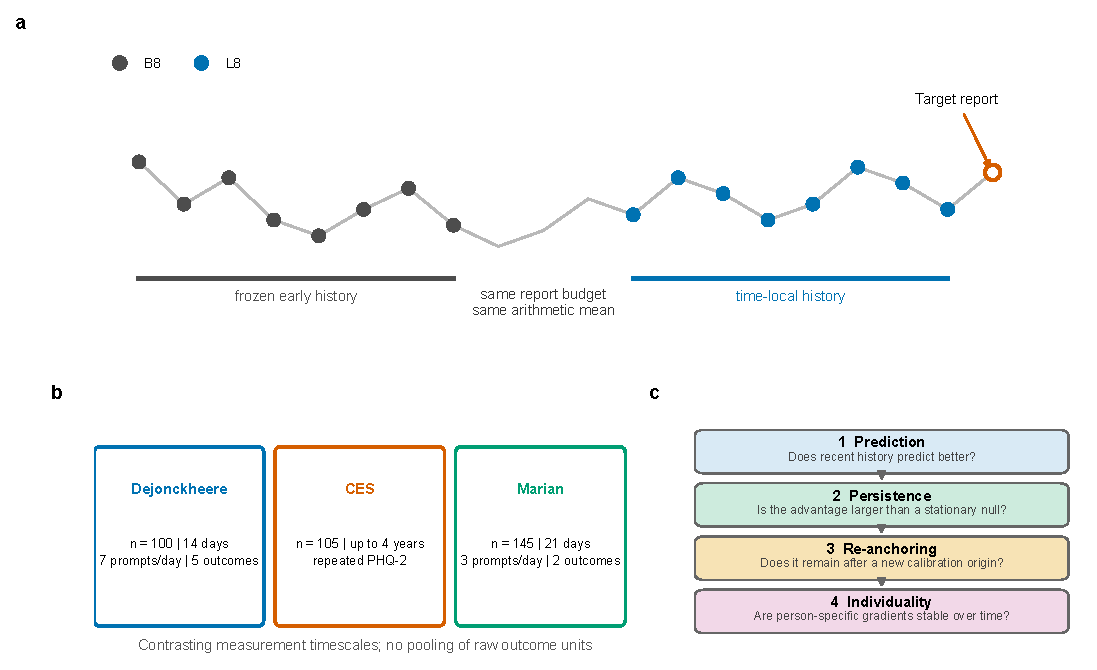
\includegraphics[width=\textwidth]{figures/Figure_1_study_design.pdf}
\caption{Study design and evidential chronology. \textbf{a}, B8 and L8 used the same number of strictly prior reports and the same arithmetic-mean estimator; only the temporal location of the reports differed. \textbf{b}, The datasets spanned dense 14--21-day experience sampling and sparse multi-year symptom assessment. \textbf{c}, CES and Marian supported development, Dejonckheere supplied an outcome-association-blind external test, and null-model, temporal-stability, prediction, sustained-change, window, recall-gap, inverse-observation-weighting, and pseudo-origin analyses were staged challenges. The figure does not imply that the complete study was preregistered.}
\label{fig:design}
\end{figure*}

\begin{table*}[!htbp]
\caption{Evidential chronology and inferential role of the analyses.}\label{tab:chronology}
\centering\small
\begin{tabularx}{\textwidth}{@{}>{\raggedright\arraybackslash}p{2.4cm}>{\raggedright\arraybackslash}p{2.8cm}>{\raggedright\arraybackslash}X>{\raggedright\arraybackslash}X@{}}
\toprule
Stage & Data & Timing relative to outcome inspection & Inferential role \\
\midrule
Development & CES and Marian & Initial patterns informed the equal-information question & Mechanism development; not confirmatory \\
External test & Dejonckheere & Outcomes, history budget, estimands, bootstrap, missingness check, and success rule were frozen before outcome associations were inspected & Outcome-association-blind, protocol-frozen external test of B8 versus L8 and the original-start age gradient \\
Cross-timescale extension & CES and Marian & Equal-information specifications were frozen after the Dejonckheere result & Tests whether the measurement pattern extends across different schedules and constructs; not an independent preregistered replication \\
Staged robustness & All applicable datasets & Added after group-level findings or in response to review under dated analysis protocols & Null models, comparators, bounded scores, temporal stability, exploratory prediction, stress test, window length, recall gap, IPW, and pseudo-origins; interpreted as secondary or post-hoc sensitivity analyses \\
\bottomrule
\end{tabularx}
\end{table*}

\subsection{Data sources and participants}

\textbf{Dejonckheere/openESM 0012.} The harmonized dataset contains 100 participants from a community sample, 9,800 scheduled rows over 14 days, and seven stratified-random prompts per day \cite{ref13,ref16}. Across the retained outcomes, 8,702 reports were complete (88.8\%). Momentary happiness, relaxation, sadness, anger, and stress were scored from 0 (not at all) to 100 (very much). Every participant contributed at least nine complete reports for each retained outcome. After the first eight complete observations, each outcome had 7,902 observed targets. Sadness and stress were the protocol-frozen primary outcomes; the other three were secondary outcomes.

\textbf{College Experience Study.} CES followed undergraduate students with repeated smartphone-based assessments over four years \cite{ref11}. The constructed PHQ-2 panel contained 5,407 complete assessments from 110 participants. We analysed the two PHQ-2 items as a 0--6 score referring to the previous two weeks. The equal-information analysis included 105 participants with at least nine complete PHQ-2 assessments and 4,541 post-calibration targets. The within-person slope analysis required at least five targets and age variation, leaving 99 participants and 4,523 targets. Public demographic fields were available for 104 of the 105 analytic participants (67.6\% female, 30.5\% male, 1.0\% coded ``both'', and 1.0\% missing; 61.9\% were coded White and 22.9\% Asian). PHQ-2 is a symptom screener rather than a clinical diagnosis. The constructed panel did not permit a fully comparable opportunity-level nonresponse denominator, so CES completion should not be compared directly with the two scheduled EMA grids.

\textbf{Marian/openESM 0052.} The harmonized dataset contains 145 undergraduate students observed over 21 days on a 9,135-row, 63-opportunity grid \cite{ref12,ref17}. We retained 8,231 complete responses (status 1; 90.1\%) to the anhedonia and depressed-mood items, each scored on four ordered categories. These items were adapted for momentary assessment and are not interchangeable with the standard PHQ-2. Every participant contributed at least nine complete reports; after the first eight, each outcome had 7,071 observed targets. Depressed mood was the primary replication outcome and anhedonia was secondary.

The analytic samples condition on providing at least eight complete reports and at least one subsequent complete target. Consequently, the analyses describe participants who remained observable beyond calibration; they do not estimate performance for people who disengaged earlier. In CES, all post-calibration targets occurred at least 14 days after the immediately preceding complete assessment, so the target PHQ-2 recall period did not overlap the nearest history assessment.

\subsection{Frozen and recent personal baselines}

For participant $i$, let $y_{ij}$ be the $j$th complete report in chronological order. The frozen early baseline was

\begin{equation}
B8_i = \frac{1}{8}\sum_{j=1}^{8} y_{ij}.
\label{eq:b8}
\end{equation}

For a target at complete-report index $t>8$, the recent rolling baseline was

\begin{equation}
L8_{it} = \frac{1}{8}\sum_{j=t-8}^{t-1} y_{ij}.
\label{eq:l8}
\end{equation}

Both predictors therefore contained exactly eight strictly prior values and used the same arithmetic-mean estimator. The current target and all future observations were unavailable when constructing either baseline. $B8_i$ remained unchanged for all later targets, whereas $L8_{it}$ moved forward by one complete observation. Earlier training-fold-weighted variants that combined the window mean with the most recent report were retained as supporting analyses; the equal-weight comparison in Eqs.~\ref{eq:b8}--\ref{eq:l8} was chosen for the clearest common interpretation.

For each target, update benefit was

\begin{equation}
U_{it}=|y_{it}-B8_i|-|y_{it}-L8_{it}|,
\label{eq:update}
\end{equation}

so that positive values indicate lower absolute error for the recent baseline.

\subsection{Baseline age and within-person slopes}

Baseline age measured how far each target lay from the participant's eighth complete report. CES used elapsed days. Dejonckheere and Marian lacked comparable raw notification timestamps in the harmonized releases, so age was the difference in scheduled opportunity counter. Within each dataset--outcome pair, age was transformed with $\log(1+\mathrm{age})$ and divided by its target-level standard deviation. This scaling supports within-outcome interpretation; raw slope magnitudes were not pooled across instruments.

For every participant with at least five eligible targets and variation in age, we fitted an ordinary least-squares slope of $U_{it}$ on that participant's mean-centred standardized age. The group summary was the arithmetic mean of these participant-specific slopes, so participants rather than repeated observations received equal weight. Five targets permit slope estimation but provide limited within-person precision; the slopes were therefore treated as secondary descriptions of the group pattern, not as reliable personal traits. We also recorded the proportion of participants with positive slopes and tested temporal stability in non-overlapping blocks.

Participant-balanced mean absolute error (MAE) and root mean squared error (RMSE) were calculated by first computing each error metric within participant and then averaging across participants. Relative error change was $(\mathrm{L8}-\mathrm{B8})/\mathrm{B8}\times100\%$; negative values favour L8.

\subsection{Post-review comparator and bounded-score analyses}

In response to methodological review, we added three strictly prior, leakage-safe descriptive comparators. The last-observation predictor used $y_{i,t-1}$. The cumulative predictor averaged all complete reports before the target. The exponentially weighted predictor (EWM8) used the fixed smoothing constant $\alpha=2/(8+1)$, was initialized at B8, and was updated only after the current target had been scored; its effective memory was therefore similar to an eight-report window without a hard cut-off. Parameters were not tuned to any outcome. These analyses were conducted after the primary findings and are labelled post-review robustness analyses rather than confirmatory tests.

For PHQ-2 and the two four-category Marian items, we additionally rounded B8 and L8 predictions to the nearest admissible category or total score and compared exact accuracy, accuracy within one score point, and ordinal absolute error. These category-level summaries test whether the B8--L8 direction survives bounded scoring; they are not latent-variable or measurement-invariance analyses. We also tabulated score means, standard deviations, floor and ceiling frequencies, source rows, complete records, and exclusions. All added intervals used 2,000 participant bootstrap resamples with the same seed and equal-participant estimand as the primary analysis.

\subsection{Null models and sensitivity analyses}

CES and Marian first underwent 500 participant-internal time permutations. Each permutation retained assessment positions, missingness, participant score distributions, target counts, and folds while randomly reordering non-missing scores. These tests asked whether the observed slope depended on temporal ordering.

Because a complete permutation also destroys short-range dependence, all eight outcomes subsequently underwent 500 non-zero participant-internal circular shifts. Circular shifts preserve each participant's score multiset, missing positions, and cyclic adjacent-pair structure but randomly relocate the study starting point. For each shift, B8, L8, update benefit, and the mean slope were reconstructed. The one-sided Monte Carlo value was $(1+k)/501$, where $k$ was the number of null slopes at least as large as the observed slope. The four primary outcomes---Dejonckheere sadness, Dejonckheere stress, CES PHQ-2, and Marian depressed mood---used a Bonferroni threshold of $0.0125$. Circular shifting introduces one artificial wrap-around adjacency and therefore approximates rather than perfectly preserves linear autocorrelation.

Dejonckheere additionally used an inverse-probability-of-observation sensitivity analysis. Completion was modelled among training participants from strictly prior completion history, study day, and prompt number; predicted probabilities were truncated to 0.10--0.99. This analysis depends on a missing-at-random assumption conditional on observed history and cannot recover unreported psychological states.

\subsection{Post-review origin, window, and observation sensitivities}

Four additional analyses were fixed in a dated protocol before execution and are reported as post-review sensitivities, not as preregistered confirmation. First, CES targets were divided by whether the gap from the immediately preceding complete assessment was below or at least 14 days; in practice, every scored target met the latter criterion. Second, Marian equal-weight B8/L8 targets were reweighted by participant-disjoint response probabilities estimated from strictly prior completion rate, missing streak, study day, and prompt number. Probabilities were truncated to 0.10--0.99 and weights were normalized within participant. Third, early and recent equal-weight means were compared for window lengths $K\in\{4,6,8,12\}$ on an identical target set beginning after 12 complete reports.

Fourth, we repeated the analysis after defining early, middle, and late pseudo-origins within each participant's complete-report sequence. Each pseudo-origin used eight reports for B8, omitted the next eight reports from evaluation, and required at least five later targets. The washout removed the mechanically identical first B8 and L8 prediction. We estimated both relative MAE and participant-specific age slopes from each origin. Origin placement depended on the retrospectively observed complete-series length, and origins shared participants and observations. This diagnostic therefore tests sensitivity to the original study start; it is neither an independent replication nor prospective rolling-origin validation.

\subsection{Temporal generalizability of individual slopes}

To test whether baseline-loss rates were stable personal characteristics, each eligible participant's post-calibration targets were divided chronologically into non-overlapping early and late halves, with at least five targets per half. Update-benefit slopes were estimated separately within each block. We calculated participant-level Pearson and Spearman correlations between early- and late-block slopes, with 2,000 participant-bootstrap resamples for the Pearson interval. A frozen gate required all four primary correlations to be positive with lower interval bounds above zero before stable individual slope prediction would be considered.

\subsection{Exploratory prediction of mean update benefit}

After the slope-generalizability result, we tested a narrower question: could the first eight reports identify participants who would obtain greater average L8 benefit in the late block? Four features were fixed: the mean, sample standard deviation, mean absolute successive difference, and linear trend across the first eight reports. A ridge model was compared with the training-fold mean using five-fold participant-held-out evaluation and nested five-fold selection of $\alpha\in\{0.01,0.1,1,10,100\}$. All feature scaling and tuning occurred inside training data. Four primary outcomes underwent 500 complete label-permutation refits and Bonferroni correction. A task passed only if RMSE improved by more than 10\%, the participant-bootstrap 95\% interval excluded zero, the out-of-fold correlation was positive, and the one-sided permutation value was no greater than 0.0125.

\subsection{Sustained-change signal-retention stress test}

We added a post-hoc semi-synthetic structural stress test to examine a failure mode that ordinary prediction error cannot reveal. For each participant with at least 32 post-calibration targets, worsening began at the midpoint of the observed sequence, increased linearly to one outcome-specific within-person standard deviation over eight complete reports, and then remained at that level for eight reports. The four primary outcomes---sadness, stress, PHQ-2, and depressed mood---all increased in the worsening direction. The observed sequence, missingness pattern, and residual variation were otherwise retained. The test quantifies how the reference rules algebraically absorb an imposed trajectory; it does not estimate diagnostic sensitivity, clinical safety, or treatment benefit.

In addition to B8 and L8, we evaluated an anchored baseline

\begin{equation}
A50_{it}=0.5B8_i+0.5L8_{it},
\label{eq:a50}
\end{equation}

whose weight was fixed before viewing the stress-test results. Injected L8 values were reconstructed using only preceding injected offsets; the current and future offsets were unavailable to the current baseline. The primary signal-retention estimand was the mean injection-induced change in worsening-direction deviation during the eight-report plateau, divided by the imposed shift. A methodological alarm threshold was estimated separately for each outcome and baseline from the participant-balanced 95th percentile of pre-injection deviation scores. We report matched future false-alarm rate, injected detection rate, their difference, and censored delay. These thresholds are comparison devices, not clinical cut-offs. Sensitivity analyses crossed 0.5- and 1.0-SD shifts, 40\%, 50\%, and 60\% onset positions, and 4-, 8-, and 16-report ramps (Supplementary Methods 4 and Tables S6--S7).

\subsection{Uncertainty, multiplicity, and software}

Unless otherwise stated, 95\% intervals were obtained from 2,000 percentile bootstrap samples of participants. Bootstrap intervals describe uncertainty among the observed participants while holding the selected datasets and analysis decisions fixed; they are not random-dataset generalization intervals. The eight B8--L8 error contrasts are reported as complete, descriptive outcome estimates rather than as a multiplicity-controlled confirmatory family. The confirmatory null-model family comprised the circular-shift tests for sadness, stress, PHQ-2, and depressed mood, with Bonferroni control at $0.05/4=0.0125$. Secondary and post-hoc analyses were interpreted from effect direction, interval width, and consistency rather than relabelled as confirmatory results. Monte Carlo values were reported to the resolution supported by 500 shifts. Exact participant and target counts are reported together throughout. Because these were fixed secondary datasets, no prospective power calculation determined sample size; eligibility and released-data availability determined $n$, and precision is conveyed by the participant-bootstrap intervals.

Analyses used Python 3.12, pandas 2.3.3, NumPy 2.3.5, scikit-learn 1.7.2, and matplotlib, with random seed 20260918. Automated tests checked temporal ordering, current/future-label exclusion, participant separation, equal-history construction, common targets across window lengths, pseudo-origin washout, semi-synthetic injection ordering, permutation invariants, participant-level resampling, and output reconciliation. Full formulas, robustness specifications, software environment, cohort flow, absolute performance, bounded-score results, and major-revision sensitivities are reported in Supplementary Methods 2--7 and Supplementary Tables S1--S15.

\section{Results}

\subsection{Recent eight-report baselines reduced prediction error}

Across all eight analysed outcomes, L8 had lower participant-balanced error than B8 (Table~\ref{tab:main}). Absolute MAE ranged from 9.58 to 17.25 points for L8 on the 0--100 Dejonckheere scales, 0.75 on the 0--6 PHQ-2 scale, and 0.38--0.40 on the 1--4 Marian scales. Relative MAE reductions ranged from 9.97\% for sadness to 29.80\% for anhedonia. CES PHQ-2 showed a 23.38\% reduction despite a substantially longer and sparser observation period than either EMA dataset. Every participant-bootstrap interval for relative MAE and RMSE change excluded zero. These eight intervals provide complete outcome-level estimates and were not treated as a multiplicity-controlled confirmatory family; the four-outcome circular-shift family supplied the prespecified null-model tests. Absolute RMSE estimates and intervals are reported in Supplementary Table S9.

\begin{table*}[!htbp]
\caption{Equal-information comparison of recent and frozen personal baselines.}\label{tab:main}
\centering
\small
\resizebox{\textwidth}{!}{%
\begin{tabular}{@{}llrrccc@{}}
\toprule
Dataset & Outcome & Participants & Targets & B8 MAE (95\% CI) & L8 MAE (95\% CI) & MAE change, \% (95\% CI)\\
\midrule
Dejonckheere & Sadness & 100 & 7,902 & 11.79 (10.47, 13.13) & 10.61 (9.48, 11.74) & $-9.97$ ($-14.95$, $-4.75$)\\
Dejonckheere & Stress & 100 & 7,902 & 21.09 (19.54, 22.62) & 17.24 (16.10, 18.43) & $-18.27$ ($-22.25$, $-14.13$)\\
Dejonckheere & Happiness & 100 & 7,902 & 17.82 (16.45, 19.19) & 14.49 (13.60, 15.38) & $-18.70$ ($-23.96$, $-13.31$)\\
Dejonckheere & Relaxation & 100 & 7,902 & 21.00 (19.73, 22.35) & 17.25 (16.31, 18.21) & $-17.82$ ($-21.91$, $-13.51$)\\
Dejonckheere & Anger & 100 & 7,902 & 10.67 (9.34, 12.04) & 9.58 (8.57, 10.57) & $-10.21$ ($-16.11$, $-3.78$)\\
CES & PHQ-2 & 105 & 4,541 & 0.97 (0.85, 1.11) & 0.75 (0.66, 0.83) & $-23.38$ ($-30.39$, $-16.26$)\\
Marian & Depressed mood & 145 & 7,071 & 0.53 (0.47, 0.59) & 0.38 (0.34, 0.42) & $-27.95$ ($-33.44$, $-21.87$)\\
Marian & Anhedonia & 145 & 7,071 & 0.57 (0.51, 0.63) & 0.40 (0.35, 0.44) & $-29.80$ ($-35.25$, $-24.11$)\\
\bottomrule
\end{tabular}%
}
\begin{flushleft}\footnotesize Negative changes indicate lower participant-balanced error for L8 than B8. Intervals use 2,000 percentile bootstrap resamples of participants. Outcomes are not commensurate and raw errors are not pooled.\end{flushleft}
\end{table*}

Figure~\ref{fig:effects} places the error contrasts and outcome-standardized age slopes on common visual scales. The plot standardizes slope magnitudes by each outcome's pooled within-person standard deviation for display only; inferential values in Table~\ref{tab:slope} remain in outcome-specific units.

\begin{figure*}[!htbp]
\centering
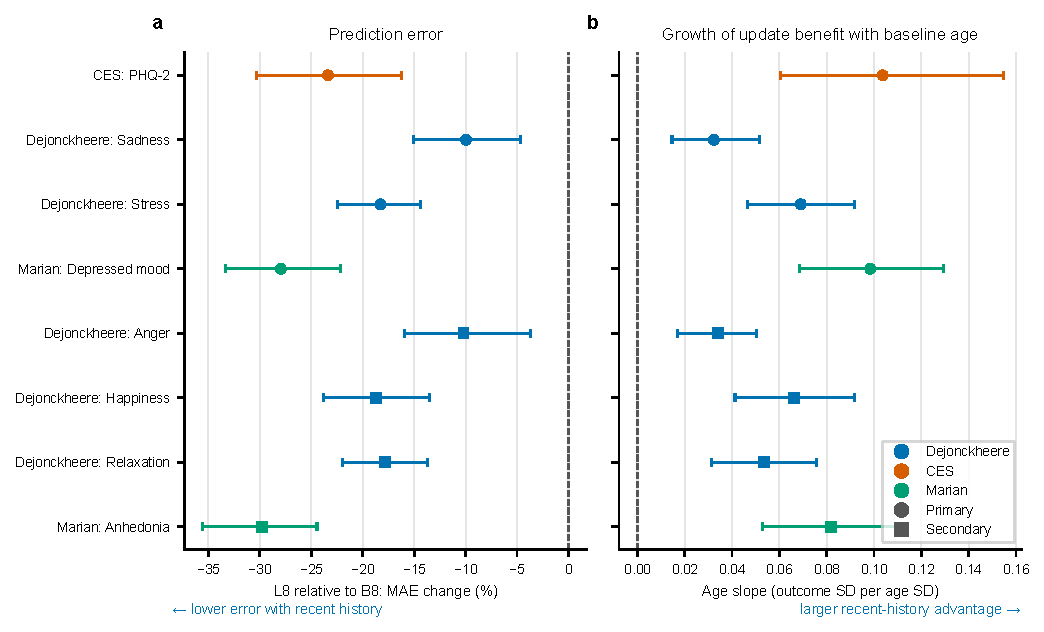
\includegraphics[width=\textwidth]{figures/Figure_2_cross_dataset_effects.pdf}
\caption{Cross-dataset prediction and baseline-age effects. \textbf{a}, Participant-balanced relative MAE change for L8 versus B8; negative values favour the recent baseline. \textbf{b}, Mean participant-specific age slope divided by the outcome's pooled within-person standard deviation. Points are outcome estimates and horizontal intervals are 95\% participant-bootstrap intervals (2,000 resamples). Circles identify the four primary outcomes and squares identify secondary outcomes. Participants, not repeated targets, were the resampling unit; exact participant and target counts are in Tables~\ref{tab:main}--\ref{tab:slope}.}
\label{fig:effects}
\end{figure*}

\subsection{Recent history reduced error but did not identify a uniquely optimal rule}

The post-review comparisons qualified the primary finding (Table~\ref{tab:comparators}). L8 outperformed the last observation for all five Dejonckheere outcomes, but not for the sparse CES and Marian measures. L8 also outperformed the cumulative personal mean for stress, happiness, relaxation, PHQ-2, depressed mood, and anhedonia; sadness and anger were inconclusive. Most importantly, fixed EWM8 had 2.05\%--3.31\% lower MAE than L8 for every outcome, with all participant-bootstrap intervals excluding zero. Thus, the B8--L8 result diagnoses loss of relevance in a start-anchored reference; it does not show that a hard eight-report rolling window is optimal.

\begin{table*}[!htbp]
\caption{Post-review leakage-safe comparison with the recent eight-report baseline.}\label{tab:comparators}
\centering\small
\resizebox{\textwidth}{!}{%
\begin{tabular}{@{}llccc@{}}
\toprule
Dataset & Outcome & L8 vs last observation, \% & L8 vs cumulative mean, \% & L8 vs EWM8, \%\\
\midrule
Dejonckheere & Sadness & $-4.53$ ($-7.08$, $-1.99$) & $-1.71$ ($-4.33$, 0.78) & 3.21 (2.44, 3.96)\\
Dejonckheere & Stress & $-6.94$ ($-9.35$, $-4.33$) & $-7.29$ ($-9.16$, $-5.53$) & 2.29 (1.69, 2.96)\\
Dejonckheere & Happiness & $-11.71$ ($-13.84$, $-9.58$) & $-4.21$ ($-6.46$, $-2.09$) & 2.72 (2.02, 3.41)\\
Dejonckheere & Relaxation & $-11.86$ ($-13.80$, $-9.82$) & $-4.81$ ($-7.02$, $-2.81$) & 2.34 (1.68, 3.07)\\
Dejonckheere & Anger & $-9.27$ ($-11.37$, $-7.06$) & $-1.54$ ($-4.11$, 1.12) & 2.05 (1.41, 2.76)\\
CES & PHQ-2 & 3.45 ($-1.65$, 9.83) & $-8.30$ ($-12.77$, $-4.63$) & 3.18 (2.09, 4.31)\\
Marian & Depressed mood & 12.98 (8.54, 17.41) & $-13.30$ ($-16.28$, $-10.71$) & 3.31 (2.34, 4.29)\\
Marian & Anhedonia & 10.46 (5.79, 15.71) & $-13.48$ ($-17.12$, $-10.14$) & 2.43 (1.56, 3.32)\\
\bottomrule
\end{tabular}%
}
\begin{flushleft}\footnotesize Values are participant-balanced relative MAE changes, $(\mathrm{L8}-\mathrm{comparator})/\mathrm{comparator}\times100\%$, with 2,000 participant-bootstrap 95\% intervals. Negative values favour L8; positive values favour the named comparator. EWM8 is a fixed exponentially weighted mean with $\alpha=2/9$. These analyses were added after review and are descriptive robustness results.\end{flushleft}
\end{table*}

Rounding predictions to admissible scores supported the B8--L8 direction for bounded outcomes. Exact accuracy increased by 9.49 percentage points for PHQ-2, 15.66 for depressed mood, and 14.83 for anhedonia; ordinal MAE decreased by 0.25, 0.18, and 0.17 score points, respectively. All corresponding participant-bootstrap intervals excluded zero (Supplementary Table S10). Strong floor concentrations---48.8\% for PHQ-2, 71.5\% for depressed mood, and 65.5\% for anhedonia---remain an important interpretive limitation (Supplementary Table S11).

\subsection{The advantage of updating increased with baseline age}

The mean within-person association between baseline age and update benefit was positive for all eight outcomes (Table~\ref{tab:slope}). For the four primary outcomes, mean slopes were 0.533 for sadness, 1.568 for stress, 0.110 for PHQ-2, and 0.059 for momentary depressed mood; each participant-bootstrap interval excluded zero. The units are outcome-specific absolute-error points per one-standard-deviation increase in log baseline age and should not be compared as standardized effect sizes across scales.

Descriptive strata showed the same pattern. In CES, the MAE advantage of L8 over B8 increased from approximately 10.7\% within 90 days of the eighth report to 39.9\% beyond 730 days. For Marian depressed mood, it increased from 19.2\% in the earliest opportunity stratum to 49.8\% in the latest. In Dejonckheere, sadness improved by 4.5\% in the earliest stratum and 18.7\% in the latest; stress improved by 7.0\% and 27.4\%, respectively. These strata were descriptive; the continuous within-person slopes were the inferential quantities.

\begin{table*}[!htbp]
\caption{Within-person baseline-age slopes and circular-shift challenges.}\label{tab:slope}
\centering
\small
\resizebox{\textwidth}{!}{%
\begin{tabular}{@{}llrrccc@{}}
\toprule
Dataset & Outcome & Participants & Targets & Mean slope (95\% CI) & Positive slopes & Circular-shift $p$\\
\midrule
Dejonckheere & Sadness$^{a}$ & 100 & 7,902 & 0.533 (0.241, 0.849) & 59.0\% & 0.005988\\
Dejonckheere & Stress$^{a}$ & 100 & 7,902 & 1.568 (1.060, 2.081) & 66.0\% & 0.001996\\
Dejonckheere & Happiness & 100 & 7,902 & 1.275 (0.793, 1.767) & 64.0\% & 0.001996\\
Dejonckheere & Relaxation & 100 & 7,902 & 1.194 (0.703, 1.697) & 71.0\% & 0.001996\\
Dejonckheere & Anger & 100 & 7,902 & 0.523 (0.261, 0.774) & 63.0\% & 0.001996\\
CES & PHQ-2$^{a}$ & 99 & 4,523 & 0.110 (0.064, 0.163) & 59.6\% & 0.001996\\
Marian & Depressed mood$^{a}$ & 145 & 7,071 & 0.059 (0.041, 0.078) & 64.8\% & 0.001996\\
Marian & Anhedonia & 145 & 7,071 & 0.052 (0.033, 0.071) & 60.7\% & 0.001996\\
\bottomrule
\end{tabular}%
}
\begin{flushleft}\footnotesize Slopes quantify the change in $|y-B8|-|y-L8|$ per one-standard-deviation increase in within-person-centred $\log(1+\mathrm{baseline\ age})$. Positive values favour L8 increasingly as B8 ages. $^{a}$Primary circular-shift family; Bonferroni threshold $p\leq0.0125$.\end{flushleft}
\end{table*}

\subsection{Temporal structure, not only local continuity, contributed to the effect}

In CES and Marian, participant-internal time permutation produced null slope means close to zero, and the observed primary slopes exceeded all 500 permuted values (one-sided $p_{\mathrm{MC}}=0.002$ for each). Circular shifting provided a more demanding challenge because it preserved cyclic adjacent-pair structure. The circular null means were positive, consistent with a contribution from short-range continuity, but remained below the observed slopes. All four primary outcomes passed the Bonferroni threshold: sadness $p_{\mathrm{MC}}=0.006$ and stress, PHQ-2, and depressed mood each $p_{\mathrm{MC}}=0.002$. All four secondary outcomes were directionally consistent. With 500 shifts, the minimum attainable corrected Monte Carlo numerator was $1/501$. These nulls show that the result was not reproduced by marginal score distributions and a cyclic approximation to local continuity alone. They do not distinguish baseline ageing from secular trend, study adaptation, seasonal context, regression after an unusual initial period, or higher-order nonstationarity.

In Dejonckheere, inverse-probability weighting for observed responses changed neither primary direction nor inference. The unweighted and weighted slopes were 0.565 versus 0.568 for sadness and 1.496 versus 1.519 for stress in the training-weighted supporting analysis. This sensitivity addresses selection conditional on observed history, not the unobserved values of missed reports.

\subsection{Error reduction survived window and observation checks, but the age gradient weakened after re-anchoring}

The recent-history error advantage was not unique to an eight-report window (Fig.~\ref{fig:robustness}a). On common targets after report 12, relative MAE changes favoured recent history for each of $K=4,6,8,$ and 12 in the four primary outcomes: sadness ranged from $-9.23\%$ to $-11.21\%$, stress from $-15.71\%$ to $-19.38\%$, PHQ-2 from $-22.82\%$ to $-29.00\%$, and depressed mood from $-23.98\%$ to $-37.89\%$. The full eight-outcome grid was directionally concordant, although the intervals for anger at $K=4$ and 6 narrowly crossed zero (Supplementary Table S13).

Observation-process checks also preserved the principal error contrast (Fig.~\ref{fig:robustness}c). Every CES target was at least 14 days after the previous complete PHQ-2 assessment; within this non-overlapping-recall sample, L8 reduced MAE by 23.38\% (95\% CI 16.62\%--30.42\%). In Marian, inverse-observation weighting changed the depressed-mood contrast from $-27.95\%$ to $-28.32\%$ and the anhedonia contrast from $-29.80\%$ to $-30.07\%$. These IPW estimates remain conditional on the observed-history missing-at-random model.

Resetting the calibration origin produced a more qualified result (Fig.~\ref{fig:robustness}b). At late origins, recent history still reduced MAE for stress ($-11.59\%$, 95\% CI $-20.28\%$ to $-2.70\%$), PHQ-2 ($-13.69\%$, $-21.55\%$ to $-5.02\%$), and depressed mood ($-21.42\%$, $-33.99\%$ to $-8.11\%$); the sadness contrast was imprecise ($-7.67\%$, $-20.35\%$ to 6.01\%). By contrast, late-origin age-slope intervals crossed zero for sadness, stress, and PHQ-2, and the anhedonia slope was negative. Middle-origin slopes were also less consistent than original-start slopes. Thus, the error advantage of recent information was more reproducible than the claim that this advantage continually increases with reference age. The original age gradient should be interpreted partly as start-related study position, not as a general decay law.

\begin{figure*}[!htbp]
\centering
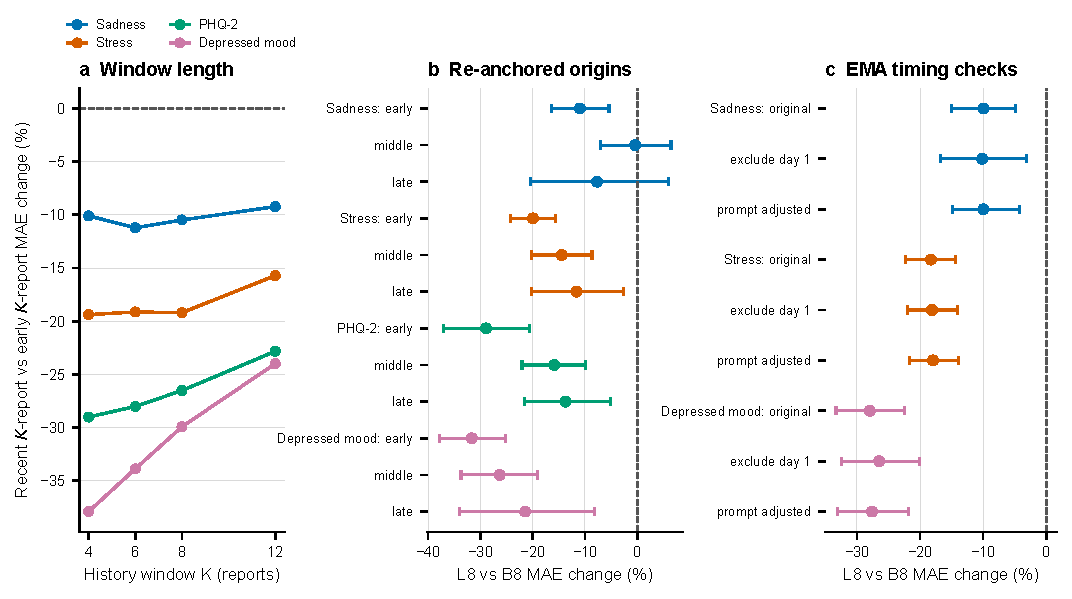
\includegraphics[width=\textwidth]{figures/Figure_5_major_revision_robustness.pdf}
\caption{Post-review robustness analyses. \textbf{a}, Participant-balanced relative MAE change for recent versus early equal-weight means across 4-, 6-, 8-, and 12-report histories on common targets after report 12. Lines show the four primary outcomes; all eight outcomes are reported in Supplementary Table S13. \textbf{b}, L8 versus B8 relative MAE change after early, middle, and late within-person pseudo-origins. Each origin used eight calibration reports, an eight-report washout, and at least five evaluation targets. \textbf{c}, Marian depressed-mood contrasts without and with inverse-observation weighting, and the CES contrast among targets separated from the previous PHQ-2 assessment by at least 14 days. Points are estimates and horizontal bars are 95\% participant-bootstrap intervals (2,000 resamples); negative values favour recent history. These post-review analyses are sensitivity checks rather than independent confirmations.}
\label{fig:robustness}
\end{figure*}

\subsection{The group pattern was not a universal individual pattern}

Although every mean slope was positive, only 59.0\%--71.0\% of participants had positive slopes in the equal-weight analyses. The average finding therefore did not describe every participant. More importantly, participant-specific slope ranks did not persist across non-overlapping time blocks. Early--late Pearson correlations were $-0.100$ (95\% CI $-0.378$ to 0.192) for sadness, $-0.084$ ($-0.305$ to 0.159) for stress, $-0.279$ ($-0.447$ to $-0.098$) for PHQ-2, and 0.086 ($-0.185$ to 0.337) for depressed mood. None passed the frozen reliability gate.

By contrast, participants' \emph{mean} update benefit was more stable across early and late blocks: Pearson correlations were 0.650 for sadness, 0.496 for stress, 0.749 for PHQ-2, and 0.690 for depressed mood, with bootstrap intervals above zero. Some people therefore tended to benefit more consistently from recent than frozen history, but the rate at which this advantage changed with age was not a stable personal characteristic.

Figure~\ref{fig:heterogeneity} juxtaposes these levels of evidence. Participant-balanced update benefit increased across relative post-calibration time quartiles, but early--late slope correlations remained near or below zero while mean-benefit correlations were positive. Relative quartiles are descriptive positions within each participant's observed sequence, not shared physical-time intervals.

\begin{figure*}[!htbp]
\centering
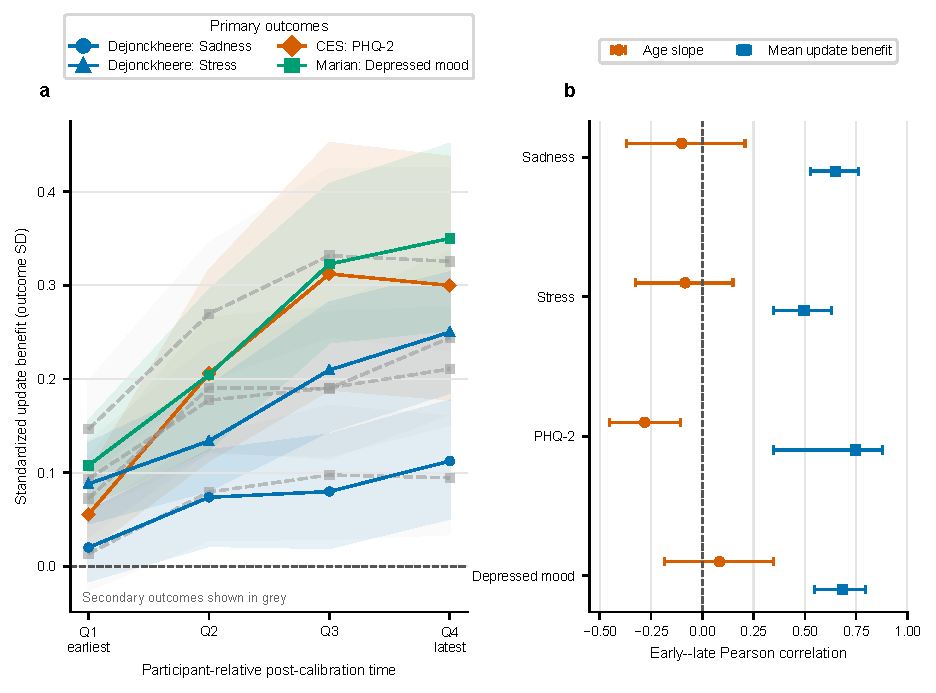
\includegraphics[width=\textwidth]{figures/Figure_3_group_and_individual_patterns.pdf}
\caption{Group-level temporal pattern and individual temporal generalizability. \textbf{a}, Participant-balanced standardized update benefit across participant-relative post-calibration time quartiles. Lines show means and shaded regions show 95\% participant-bootstrap intervals; primary outcomes are coloured and secondary outcomes are grey. \textbf{b}, Pearson correlations between non-overlapping early- and late-block estimates for the age slope and mean update benefit in the four primary outcomes. Points show correlations and horizontal intervals show 95\% participant-bootstrap intervals. The independent unit is the participant; $n=97$--145 depending on outcome.}
\label{fig:heterogeneity}
\end{figure*}

\subsection{Early reports predicted update benefit only for selected outcomes}

The exploratory ridge analysis yielded construct-dependent results (Supplementary Table S5). First-eight-report summaries predicted late-block mean update benefit for sadness and depressed mood under the frozen gate, reducing RMSE by 10.40\% and 14.48\%, respectively. Stress and PHQ-2 did not improve meaningfully over the training-fold mean. The first-eight mean had positive coefficients in every outer fold for the two passing outcomes, whereas variability and trend coefficients were smaller and inconsistent. Because the first-eight mean also defines B8, this pattern can include scale boundaries, regression to the mean, and mathematical coupling; it should not be interpreted as a stable psychological trait or as evidence that machine learning is required.

\subsection{Rolling baselines traded prediction accuracy for sustained-change signal retention}

The semi-synthetic structural stress test exposed a limitation that was not visible from MAE alone (Fig.~\ref{fig:safety}). Under the primary eight-report ramp and eight-report plateau, B8 retained the entire imposed plateau deviation by construction. L8 retained 16.4\%, because the recent window had incorporated most of the worsening, whereas A50 retained 58.2\%. These retention values were identical across outcomes because they follow algebraically from the fixed window, ramp, and anchor; they are properties of the imposed scenario and reference rules, not empirically estimated clinical sensitivities.

The accuracy side of the trade-off was data-dependent. Across the four primary outcomes, A50 reduced original-data participant-balanced MAE by 8.79\%--16.42\% relative to B8 and preserved 58.8\%--88.2\% of the full L8 gain. The methodological alarm analysis was less decisive: excess alarm rates were 3.19--10.06 percentage points for B8, 1.19--2.06 points for L8, and 2.88--5.02 points for A50. Results across the complete amplitude, onset, and ramp grid preserved the ordering B8 $>$ A50 $>$ L8 for signal retention; slower ramps reduced retention further (Supplementary Table S7). Thus, A50 occupied an intermediate accuracy--retention position, but neither it nor the alarm rule received prospective or clinical validation.

\begin{figure*}[!htbp]
\centering
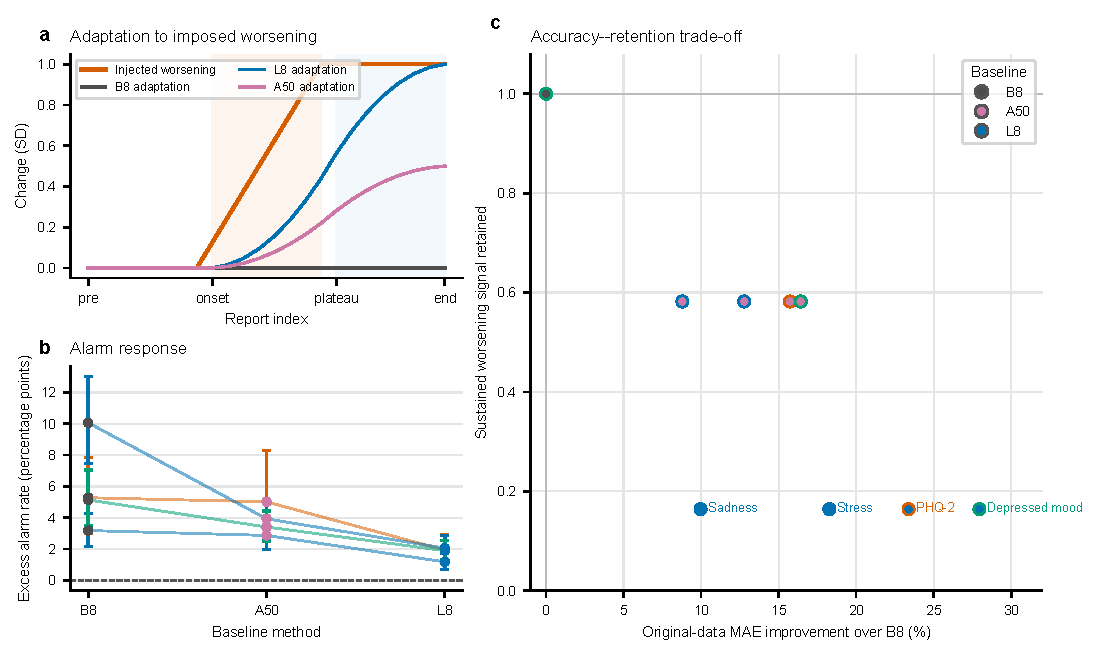
\includegraphics[width=\textwidth]{figures/Figure_4_accuracy_signal_tradeoff.pdf}
\caption{Semi-synthetic sustained-change structural stress test. \textbf{a}, Primary injection schedule and deterministic adaptation of B8, L8, and A50. \textbf{b}, Injected minus matched-original alarm rate under thresholds derived from the participant-balanced pre-injection 95th percentile; points are outcome estimates and intervals are 95\% participant-bootstrap intervals. \textbf{c}, Original-data participant-balanced MAE improvement versus sustained plateau signal retained for each primary outcome. Discrete points show the three prespecified reference rules and should not be read as a continuous or optimized frontier. The primary scenario used a one-within-person-SD shift, an eight-report ramp, and eight plateau reports; eligible participants were 71 for PHQ-2, 100 for sadness and stress, and 141 for depressed mood. This post-hoc structural stress test is not a clinical safety, diagnostic, or treatment evaluation.}
\label{fig:safety}
\end{figure*}

\section{Discussion}

\subsection{Principal findings}

Across a sparse multi-year symptom design and two dense EMA designs, recent personal history predicted later self-reports more accurately than an equally sized early history. The error advantage appeared across eight analysed outcomes, remained across several window lengths and observation-process checks, and exceeded null distributions that preserved participant score distributions and a cyclic approximation to local sequence structure. Re-anchoring within each series preserved the late-origin advantage for stress, PHQ-2, and depressed mood but made sadness inconclusive. More importantly, the positive age gradient attenuated after re-anchoring. The strongest supported claim is therefore that an early study-start reference often loses predictive relevance, not that every personal baseline obeys a universal time-decay law. Category-level analyses supported the same direction for bounded outcomes. EWM8 was consistently slightly more accurate than L8, while the last observation was competitive for sparse or strongly floored measures; a hard eight-report window is not uniquely optimal.

The equally important negative finding concerns individuality. The group-average age gradient was not shared by everyone, and a person's estimated gradient in one time block did not predict their gradient in another. A baseline can become less useful on average without each person possessing a stable ``decay rate.'' This distinction prevents a group-level property of repeated measurement from being reified as an individual trait.

\subsection{Psychological interpretation}

Personal baselines are often introduced to respect individual differences, but a fixed baseline can become another population-like simplification if it assumes that the earlier person is an adequate reference for the later person. The present findings are consistent with a temporally local view of psychological measurement: personal history is informative, but its meaning is conditional on when it was observed. This view complements work emphasizing that within-person processes cannot be inferred directly from between-person differences and that dynamic conclusions depend on measurement timescale \cite{ref4,ref5,ref6}.

The analyses do not identify why early baselines lost relative value. CES spans academic years and the COVID-19 period, whereas the EMA studies span only two or three weeks. Change could reflect symptoms, affect regulation, context, scale use, study adaptation, regression to the mean, or selection into continued responding. B8 age is inseparable from position in the observed study, and circular shifts introduce a wrap boundary while failing to reproduce every slow trend or seasonal process. The pseudo-origin results directly reinforce this caution: error reduction often survived re-anchoring, whereas the age gradient did not. Cross-timescale convergence argues against a single dataset artifact but does not establish a common latent mechanism. We therefore use ``baseline freshness'' and ``start-related nonstationarity'' as statistical descriptions rather than causal or psychological diagnoses.

\subsection{Implications for repeated assessment and personalisation}

The main practical implication is methodological. Researchers should state whether a personal reference is frozen or updated, report how old its information is at prediction, and compare adaptive rules with simple leakage-safe heuristics. A model can appear personalised because it contains person-specific parameters while still relying on stale data. Conversely, frequent updating is not automatically preferable: an adaptive baseline may absorb a gradual and meaningful worsening into a new normal. Prediction error and sensitivity to sustained deterioration are different objectives. This interpretation agrees with recent calls to treat behavioural baselines as task- and context-specific forecasting rules and to retain an external criterion when clinically important gradual change must remain visible \cite{ref20}.

Our exploratory analysis also advises restraint in algorithm selection. Four simple summaries of the first eight reports identified later update benefit for sadness and depressed mood but not for stress or PHQ-2. With only 97--145 participants per task, deeper or more flexible models would increase the opportunity to fit unstable individual differences. The present evidence supports a modest, construct-dependent machine-learning signal rather than a general allocation algorithm.

The stress test adds a second restraint: the objective function matters. Minimizing next-report error rewards a rolling baseline for following gradual change, whereas a monitoring system may need to preserve that change as a deviation from a longer-term reference. This is not a contradiction between accurate and inaccurate models; it is a conflict between time-local prediction and sustained-change visibility. A50 illustrates one transparent way to expose the trade-off. Its fixed weight was not optimized and its intermediate performance should motivate prospective comparison rather than deployment.

\subsection{Strengths and limitations}

Strengths include the equal eight-report comparison, participant-balanced estimation, transparent evidence chronology, outcome-complete reporting, an outcome-association-blind protocol-frozen external test, multiple null models, and post-review comparison with last-observation, cumulative, and exponentially weighted references. The analysis also retained a negative reliability result that constrains the strongest personalisation claim. Automated tests verified that current and future reports did not enter the baselines and that repeated observations did not masquerade as independent participants.

Several limitations remain. First, two datasets contributed to direction development before the equal-information extension, and only Dejonckheere was outcome-association-blind for the core hypothesis. The earlier OSF registration covered another research question. The present study is therefore a staged secondary analysis, not a preregistered confirmatory study. Comparator, bounded-score, window, recall-gap, IPW, and pseudo-origin analyses were prompted by review and are explicitly post hoc. Second, outcomes, response scales, reference periods, populations, and schedules differed. This heterogeneity tests a measurement pattern but prevents pooled raw effects or claims about a common disorder. Arithmetic means still impose interval-like distances on ordinal items; category-level scoring establishes directional robustness, not measurement invariance. Third, eligibility required repeated completion. Dejonckheere and Marian retained 88.8\% and 90.1\% of scheduled rows, but included-versus-excluded participant comparisons were impossible where every released participant passed calibration, and the CES constructed panel lacked a comparable opportunity denominator. Marian and Dejonckheere IPW analyses address only modelled observation processes under conditional missing-at-random assumptions. Fourth, baseline age remains partly a study-position variable. Pseudo-origin placement depended on the retrospectively observed series length, origins shared observations, and late-origin analyses had only five targets per eligible participant. They narrow the original claim but do not constitute prospective rolling-origin validation or identify the responsible mechanism. Circular shifting creates an artificial wrap boundary and cannot reproduce every slow trend. Fifth, individual slopes have unequal precision because series lengths differ; the five-target minimum permits estimation but can produce noisy slopes. Participant bootstrap protects the equal-participant group mean but does not make an individual slope a reliable trait, so slope findings are interpreted as secondary. Finally, overlapping rolling windows can stabilize mean update benefit; the non-overlapping temporal-block analysis was necessary and showed that personal slopes were not stable.

Finally, lower prediction error does not establish clinical benefit or safety. The analyses did not test diagnostic thresholds, treatment decisions, or a randomised assessment schedule. The semi-synthetic stress test isolated one structural failure mode, but it used imposed trajectories and a methodological threshold rather than observed clinical deterioration. Its signal-retention estimates partly follow from the chosen ramp and window, and the alarm-rate contrasts were modest. Prospective event labels and externally specified action thresholds remain necessary before adaptive monitoring can be evaluated clinically.

\subsection{Future research}

A prospective test should freeze B8, L8, EWM8, one or two anchored weights, and multiple calibration origins before inspecting a new dataset. It should preserve the equal-history comparison and predefine psychologically meaningful deterioration events. Short-term prediction and sustained-change detection should be treated as co-primary objectives. A design with randomized or naturally staggered calibration origins, or trend- and autocorrelation-matched simulations, is needed to separate elapsed reference age from generic study-position effects. If the trade-off differs between participants, allocation models should be evaluated on new participants and later time blocks, not on overlapping observations from the same period.

\section{Conclusions}

Across these selected repeated-self-report samples, equally sized recent histories predicted later affect, stress, and depressive-symptom reports more accurately than early start-anchored histories. Error reduction persisted across window and observation sensitivities and often after re-anchoring, but the apparent age gradient weakened at alternative origins and was not a stable individual characteristic. EWM8 modestly outperformed the hard rolling window, while updating absorbed most of an imposed sustained deviation. Personal baselines should therefore be treated as time-local measurement summaries: when they were established, how they update, their predictive error, and their sustained-change behaviour require separate evaluation before any clinical use.

\section{List of abbreviations}

A50: equal-weight average of B8 and L8; B8: frozen mean of the first eight complete reports; CES: College Experience Study; CI: confidence interval; EMA: ecological momentary assessment; L8: rolling mean of the eight most recent complete reports; MAE: mean absolute error; PHQ-2: Patient Health Questionnaire-2; RMSE: root mean squared error.

\section{Declarations}

\subsection{Ethics approval and consent to participate}

This study was a secondary analysis of de-identified datasets and involved no new recruitment, participant contact, or intervention. The School of Mathematics and Statistics at Hanshan Normal University confirmed that, under the University's institutional requirements, no additional ethics approval was required for this secondary analysis. Ethics approval and informed-consent procedures for the original data collections are reported in the source studies \cite{ref11,ref12,ref13}.

\subsection{Consent for publication}

Not applicable.

\subsection{Availability of data and materials}

The CES dataset is described in Nepal et al. \cite{ref11} and is distributed through Kaggle (\url{https://www.kaggle.com/datasets/subigyanepal/college-experience-dataset}) under CC BY-NC-SA 4.0; access and reuse remain governed by the repository terms. Harmonized Dejonckheere/openESM 0012 data are available from Zenodo (doi:10.5281/zenodo.17347569) under CC BY 4.0 \cite{ref16}. Harmonized Marian/openESM 0052 data are available from Zenodo (doi:10.5281/zenodo.17348267) under CC BY 4.0 \cite{ref17}. Raw third-party data are not redistributed with this manuscript. The public analysis repository is \url{https://github.com/liaorunqing/psychology}. The reproducibility materials corresponding to this manuscript are archived as release v1.1.0 (\url{https://github.com/liaorunqing/psychology/releases/tag/v1.1.0}); this release includes the post-review scripts, automated tests, dated protocols, non-identifying aggregate outputs, figure source data, and LaTeX manuscript source. Readers must obtain the third-party datasets from their original repositories to rebuild participant-level analysis tables. A long-term archival DOI has not yet been assigned and is not claimed in the present version.

\subsection{Competing interests}

The authors declare that they have no competing interests.

\subsection{Funding}

This work was supported by the National Natural Science Foundation of China (Grant No. 12271132) and the Department of Education of Guangdong Province, China (Grant No. 2024ZDZX1027).

\subsection{Authors' contributions}

R.L.: Conceptualization, Data curation, Software, Formal analysis, Visualization, and Writing---original draft. Z.W.: Supervision, Methodology, Writing---review and editing, Project administration, and Funding acquisition.

\subsection{Acknowledgements}

Not applicable.

\subsection{Patient and public involvement}

Patients and members of the public were not involved in the design, analysis, reporting, or dissemination planning of this secondary-data study.

\begin{thebibliography}{99}
\bibitem{ref1} Molenaar PCM. A manifesto on psychology as idiographic science: bringing the person back into scientific psychology, this time forever. Meas Interdiscip Res Perspect. 2004;2(4):201--218. doi: \url{https://doi.org/10.1207/S15366359MEA0204_1}.
\bibitem{ref2} Hamaker EL, Wichers M. No time like the present: discovering the hidden dynamics in intensive longitudinal data. Curr Dir Psychol Sci. 2017;26(1):10--15. doi: \url{https://doi.org/10.1177/0963721416666518}.
\bibitem{ref3} Shiffman S, Stone AA, Hufford MR. Ecological momentary assessment. Annu Rev Clin Psychol. 2008;4:1--32. doi: \url{https://doi.org/10.1146/annurev.clinpsy.3.022806.091415}.
\bibitem{ref4} Neubauer AB, Schmiedek F. Studying within-person variation and within-person couplings in intensive longitudinal data: lessons learned and to be learned. Gerontology. 2020;66(4):332--339. doi: \url{https://doi.org/10.1159/000507993}.
\bibitem{ref5} Scott SB, Sliwinski MJ, Zawadzki M, et al. A coordinated analysis of variance in affect in daily life. Assessment. 2020;27(8):1683--1698. doi: \url{https://doi.org/10.1177/1073191118799460}.
\bibitem{ref6} Curran PJ, Bauer DJ. The disaggregation of within-person and between-person effects in longitudinal models of change. Annu Rev Psychol. 2011;62:583--619. doi: \url{https://doi.org/10.1146/annurev.psych.093008.100356}.
\bibitem{ref7} Myin-Germeys I, Kasanova Z, Vaessen T, et al. Experience sampling methodology in mental health research: new insights and technical developments. World Psychiatry. 2018;17(2):123--132. doi: \url{https://doi.org/10.1002/wps.20513}.
\bibitem{ref8} Aalbers G, Hendrickson AT, Vanden Abeele MMP, Keijsers L. Smartphone-tracked digital markers of momentary subjective stress in college students: idiographic machine learning analysis. JMIR Mhealth Uhealth. 2023;11:e37469. doi: \url{https://doi.org/10.2196/37469}.
\bibitem{ref9} Balliu B, Douglas C, Seok D, et al. Personalized mood prediction from patterns of behavior collected with smartphones. NPJ Digit Med. 2024;7:49. doi: \url{https://doi.org/10.1038/s41746-024-01035-6}.
\bibitem{ref10} Webb CA, Ren B, Rahimi-Eichi H, et al. Personalized prediction of negative affect in individuals with serious mental illness followed using long-term multimodal mobile phenotyping. Transl Psychiatry. 2025;15:174. doi: \url{https://doi.org/10.1038/s41398-025-03394-4}.
\bibitem{ref11} Nepal S, Liu W, Pillai A, et al. Capturing the College Experience: a four-year mobile sensing study of mental health, resilience and behavior of college students during the pandemic. Proc ACM Interact Mob Wearable Ubiquitous Technol. 2024;8(1):Article 38. doi: \url{https://doi.org/10.1145/3643501}.
\bibitem{ref12} Marian S, Costantini G, Macsinga I, Sava FA. The dynamic interplay of anxious and depressive symptoms in a sample of undergraduate students. J Psychopathol Behav Assess. 2023;45(1):150--159. doi: \url{https://doi.org/10.1007/s10862-022-10014-8}.
\bibitem{ref13} Dejonckheere E, Kalokerinos EK, Bastian B, Kuppens P. Poor emotion regulation ability mediates the link between depressive symptoms and affective bipolarity. Cogn Emot. 2019;33(5):1076--1083. doi: \url{https://doi.org/10.1080/02699931.2018.1524747}.
\bibitem{ref14} von Elm E, Altman DG, Egger M, et al. The Strengthening the Reporting of Observational Studies in Epidemiology (STROBE) statement: guidelines for reporting observational studies. PLoS Med. 2007;4(10):e296. doi: \url{https://doi.org/10.1371/journal.pmed.0040296}.
\bibitem{ref15} Collins GS, Moons KGM, Dhiman P, et al. TRIPOD+AI statement: updated guidance for reporting clinical prediction models that use regression or machine learning methods. BMJ. 2024;385:e078378. doi: \url{https://doi.org/10.1136/bmj-2023-078378}.
\bibitem{ref16} Dejonckheere E, Kalokerinos EK, Bastian B, Kuppens P. Dejonckheere (2019), harmonized experience-sampling dataset [dataset]. Zenodo; 2025. doi: \url{https://doi.org/10.5281/zenodo.17347569}.
\bibitem{ref17} Marian S, Costantini G, Macsinga I, Sava FA. Marian (2022), harmonized experience-sampling dataset [dataset]. Zenodo; 2025. doi: \url{https://doi.org/10.5281/zenodo.17348267}.
\bibitem{ref18} Stamatis CA, Meyerhoff J, Meng Y, et al. Differential temporal utility of passively sensed smartphone features for depression and anxiety symptom prediction: a longitudinal cohort study. NPJ Ment Health Res. 2024;3:1. doi: \url{https://doi.org/10.1038/s44184-023-00041-y}.
\bibitem{ref19} Allgaier J, Pryss R. Practical approaches in evaluating validation and biases of machine learning applied to mobile health studies. Commun Med. 2024;4:76. doi: \url{https://doi.org/10.1038/s43856-024-00468-0}.
\bibitem{ref20} Just SA, Tedeschi E, Holsb\o{} E, et al. The challenges of implementing hybrid baselines for the interpretation of longitudinal behavioral data from individuals. NPJ Digit Med. 2026;9:331. doi: \url{https://doi.org/10.1038/s41746-026-02668-5}.
\end{thebibliography}

\end{document}
